\subsection{The snake diagram}

PROPOSITION 1. --- Consider a commutative diagram of A-modules

\[
\begin{array}{c} \mathrm{M} \xrightarrow {u} \mathrm{N} \xrightarrow {v} \mathrm{P} \\ f \Big \downarrow \qquad \qquad \qquad g \Big \downarrow \qquad \qquad \qquad h \Big \downarrow \\ \mathrm{M} ^ {\prime} \xrightarrow {u ^ {\prime}} \mathrm{N} ^ {\prime} \xrightarrow {v ^ {\prime}} \mathrm{P} ^ {\prime}. \end{array}\tag{4}
\]

Suppose that the two rows of (4) are exact. Then:

\begin{enumerate}
\def\labelenumi{(\roman{enumi})}
\tightlist
\item
  If h is injective, we have
\end{enumerate}

\[
\operatorname{Im} (g) \cap \operatorname{Im} \left(u ^ {\prime}\right) = \operatorname{Im} \left(u ^ {\prime} \circ f\right) = \operatorname{Im} (g \circ u).\tag{5}
\]

\begin{enumerate}
\def\labelenumi{(\roman{enumi})}
\setcounter{enumi}{1}
\tightlist
\item
  If f is surjective, we have
\end{enumerate}

\[
\operatorname{Ker} (g) + \operatorname{Im} (u) = \operatorname{Ker} \left(v ^ {\prime} \circ g\right) = \operatorname{Ker} (h \circ v).\tag{6}
\]

Let us prove (i). It is clear that we have

\[
\operatorname{Im} \left(u ^ {\prime} \circ f\right) = \operatorname{Im} (g \circ u) \subset \operatorname{Im} (g) \cap \operatorname{Im} \left(u ^ {\prime}\right).
\]

Conversely, let \(y' \in \operatorname{Im}(g) \cap \operatorname{Im}(u')\) . There exists \(y \in \mathbf{N}\) such that \(y' = g(y)\) . Since \(v' \circ u' = 0\) , we have \(0 = v'(y') = v'(g(y)) = h(v(y))\) , whence \(v(y) = 0\) since \(h\) is injective. Since \((u, v)\) is an exact sequence, there exists \(x \in \mathbf{M}\) such that \(y = u(x)\) , whence \(y' = g(u(x))\) .

Let us prove (ii). Since \(v \circ u = 0\) and \(v' \circ u' = 0\) it is clear that

\[
\operatorname{Ker} (g) + \operatorname{Im} (u) \subset \operatorname{Ker} \left(v ^ {\prime} \circ g\right) = \operatorname{Ker} (h \circ v).
\]

Conversely, let \(y \in \operatorname{Ker}(v' \circ g)\) . Then \(g(y) \in \operatorname{Ker}(v')\) , and there exists \(x' \in M'\) such that \(u'(x') = g(y)\) since the sequence \((u', v')\) is exact. Since \(f\) is surjective, there exists \(x \in M\) such that \(f(x) = x'\) , whence \(g(y) = u'(f(x)) = g(u(x))\) ; from this we conclude that \(y - u(x) \in \operatorname{Ker}(g)\) , which completes the proof.

Lemma 1. --- Consider a commutative diagram of A-modules

\[
\begin{array}{c} \mathbf {M} \xrightarrow {\quad u \quad} \mathbf {N} \\ f \Big \downarrow \qquad \qquad \qquad \qquad \qquad \qquad \qquad \qquad g \Big \downarrow \\ \mathbf {M} ^ {\prime} \xrightarrow {\quad u ^ {\prime} \quad} \mathbf {N} ^ {\prime}. \end{array}\tag{7}
\]

Then there exists one and only one homomorphism \(u_1: \text{Ker}(f) \to \text{Ker}(g)\) and one and only one homomorphism \(u_2: \text{Coker}(f) \to \text{Coker}(g)\) , such that the diagrams

\[
\begin{array}{c} \operatorname{Ker} (f) \xrightarrow {u _ {1}} \operatorname{Ker} (g) \\ i \Biggl \downarrow \\ \mathrm{M} \xrightarrow [ u ]{} \mathrm{N} \end{array}\tag{8}
\]

and

\begin{enumerate}
\def\labelenumi{(\arabic{enumi})}
\setcounter{enumi}{8}
\tightlist
\item
\end{enumerate}

\pandocbounded{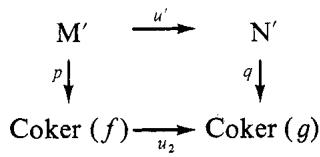
\includegraphics[keepaspectratio]{images/part001_11db974a.jpg}}

Let them be commutative, with i and j denoting the canonical injections, and p and q the canonical surjections.

Indeed, if \(x \in \operatorname{Ker}(f)\) , we have \(f(x) = 0\) and \(g(u(x)) = u'(f(x)) = 0\) , hence \(u(x) \in \operatorname{Ker}(g)\) , and the existence and uniqueness of \(u_1\) are then immediate. Likewise, we have

\[
u ^ {\prime} (f (\mathbf {M})) = g (u (\mathbf {M})) \subset g (\mathbf {N}),
\]

hence \(u'\) gives by passage to quotients a homomorphism

\[
u _ {2}: \operatorname{Coker} (f) \rightarrow \operatorname{Coker} (g),
\]

which is the unique homomorphism for which (9) is commutative.

Now start from a commutative diagram (4) of A-modules; by virtue of Lemma 1 there corresponds to it a commutative diagram

\[
\begin{array}{c c c c c} \operatorname{Ker} (f) \xrightarrow {u _ {1}} & \operatorname{Ker} (g) \xrightarrow {v _ {1}} & \operatorname{Ker} (h) \\ i \Big \downarrow & j \Big \downarrow & k \Big \downarrow \\ \mathbf {M} & u & \mathbf {N} & v & \mathbf {P} \\ f \Big \downarrow & g \Big \downarrow & h \Big \downarrow \\ \mathbf {M} ^ {\prime} & u ^ {\prime} & \mathbf {N} ^ {\prime} & v ^ {\prime} & \mathbf {P} ^ {\prime} \\ p \Big \downarrow & q \Big \downarrow & r \Big \downarrow \\ \operatorname{Coker} (f) \xrightarrow {u _ {2}} & \operatorname{Coker} (g) \xrightarrow {v _ {2}} & \operatorname{Coker} (h) \end{array}\tag{10}
\]

where \(i, j, k\) are the canonical injections, \(p, q, r\) the canonical surjections, \(u_{1}, u_{2}\) (resp. \(v_{1}, v_{2}\) ) the homomorphisms deduced from \(u\) , \(u'\) (resp. \(v, v'\) ) by Lemma 1.

PROPOSITION 2. --- Suppose that in the commutative diagram (4), the sequences \((u, v)\) and \((u', v')\) are exact. Then:

\begin{enumerate}
\def\labelenumi{(\roman{enumi})}
\item
  One has \(v_{1} \circ u_{1} = 0\) ; if \(u'\) is injective, the sequence \((u_{1}, v_{1})\) is exact.
\item
  One has \(v_2 \circ u_2 = 0\) ; if v is surjective, the sequence \((u_2, v_2)\) is exact.
\item
  Suppose \(u'\) injective and \(v\) surjective. There then exists one and only one homomorphism \(d: \operatorname{Ker}(h) \to \operatorname{Coker}(f)\) having the following property: if \(z \in \operatorname{Ker}(h)\) , \(y \in \mathbf{N}\) and \(x' \in \mathbf{M}'\) satisfy the relations \(v(y) = k(z)\) and \(u'(x') = g(y)\) , we have \(d(z) = p(x')\) . Moreover, the sequence
\end{enumerate}

(*) \(\operatorname{Ker}(f) \xrightarrow{u_1} \operatorname{Ker}(g) \xrightarrow{v_1} \operatorname{Ker}(h) \xrightarrow{d} \operatorname{Coker}(f) \xrightarrow{u_2} \operatorname{Coker}(g) \xrightarrow{v_2} \operatorname{Coker}(h)\) is exact.

\pandocbounded{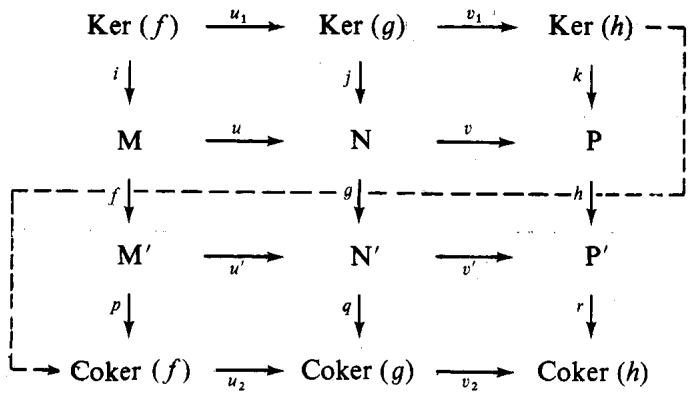
\includegraphics[keepaspectratio]{images/part001_0570902c.jpg}}

Let us prove (i). Since \(u_{1}\) and \(v_{1}\) have the same graphs as the restrictions of \(u\) and \(v\) to \(\operatorname{Ker}(f)\) and \(\operatorname{Ker}(g)\) respectively, we have \(v_{1} \circ u_{1} = 0\) . We have

\[
\operatorname{Ker} \left(v _ {1}\right) = \operatorname{Ker} (g) \cap \operatorname{Ker} (v) = \operatorname{Ker} (g) \cap \operatorname{Im} (u) = \operatorname{Im} (j) \cap \operatorname{Im} (u).
\]

But by prop. 1 (i), we have \(\operatorname{Ker}(v_1) = \operatorname{Im}(j \circ u_1) = \operatorname{Im}(u_1)\) if \(u'\) is injective. Let us prove (ii). Since \(u_2\) and \(v_2\) come from \(u\) and \(v\) by passing to quotients, it is clear that \(v_2 \circ u_2 = 0\) . Suppose \(v\) surjective; since \(q\) and \(p\) are surjective, we have, by virtue of the hypotheses and of prop. 1 (ii)

\[
\begin{array}{r l} \operatorname{Ker} (v _ {2}) & = q (\operatorname{Ker} (v _ {2} \circ q)) = q (\operatorname{Ker} (v ^ {\prime}) + \operatorname{Im} (g)) = q (\operatorname{Ker} (v ^ {\prime})) \\ & = q (\operatorname{Im} (u ^ {\prime})) = \operatorname{Im} (q \circ u ^ {\prime}) = \operatorname{Im} (u _ {2} \circ p) = \operatorname{Im} (u _ {2}). \end{array}
\]

Finally, let us prove (iii). For \(z \in \operatorname{Ker}(h)\) there exists \(y \in \mathbf{N}\) such that \(v(y) = k(z)\) since \(v\) is surjective; moreover, we have \(v'(g(y)) = h(k(z)) = 0\) and consequently there exists a unique \(x' \in \mathbf{M}'\) such that \(u'(x') = g(y)\) since \(u'\) is injective. Let us show that the element \(p(x') \in \operatorname{Coker}(f)\) is independent of the element \(y \in \mathbf{N}\) such that \(v(y) = k(z)\) . Indeed, if \(y_1 \in \mathbf{N}\) is a second element such that \(v(y_1) = k(z)\) , we have \(y_1 = y + u(x)\) where \(x \in \mathbf{M}\) . Let us show that if \(x_1' \in \mathbf{M}'\) is such that \(u'(x_1') = g(y_1)\) , we have \(x_1' = x' + f(x)\) ; indeed, we have \(u'(x' + f(x)) = u'(x') + u'(f(x)) = g(y) + g(u(x)) = g(y + u(x)) = g(y_1)\) . Finally, we conclude that \(p(x_1') = p(x') + p(f(x)) = p(x')\) . We can therefore set \(d(z) = p(x')\) and we have thus defined a map \(d: \operatorname{Ker}(h) \to \operatorname{Coker}(f)\) .

If now \(z_{1}, z_{2}\) are elements of \(\operatorname{Ker}(h)\) , if \(\lambda_{1}, \lambda_{2} \in \mathbf{A}\) and \(z = \lambda_{1} z_{1} + \lambda_{2} z_{2}\) , we take elements \(y_{1}\) and \(y_{2}\) of \(\mathbf{N}\) such that \(v(y_{1}) = k(z_{1})\) and \(v(y_{2}) = k(z_{2})\) and we choose for \(y \in \mathbf{N}\) the element \(\lambda_{1} y_{1} + \lambda_{2} y_{2}\) ; it is then immediate that

\[
d (z) = \lambda_ {1} d (z _ {1}) + \lambda_ {2} d (z _ {2}),
\]

so d is a homomorphism.

Suppose that \(z = v_1(t)\) for a \(t \in \operatorname{Ker}(g)\) ; we will then take for \(y \in \mathbf{N}\) the element \(j(t)\) . Since \(g(j(t)) = 0\) , we conclude \(d(z) = 0\) , hence \(d \circ v_1 = 0\) . Conversely, suppose that \(d(z) = 0\) . With the preceding notation, we therefore have \(x' = f(x)\) , where \(x \in M\) . In this case, we have \(g(y) = u'(f(x)) = g(u(x))\) , or equivalently \(g(y - u(x)) = 0\) . The element \(y - u(x)\) is therefore of the form \(j(n)\) for \(n \in \operatorname{Ker}(g)\) , and we have

\[
k (z) = v (y) = v (u (x) + j (n)) = v (j (n)) = k \left(v _ {1} (n)\right);
\]

since \(k\) is injective, \(z = v_{1}(n)\) , which proves that the sequence (*) is exact at \(\operatorname{Ker}(h)\) . Finally, we have (still with the same notation)

\[
u _ {2} (d (z)) = u _ {2} \left(p \left(x ^ {\prime}\right)\right) = q \left(u ^ {\prime} \left(x ^ {\prime}\right)\right) = q (g (y)) = 0 \quad \text {   hence   } \quad u _ {2} \circ d = 0.
\]

Conversely, suppose that an element \(w = p(x')\) of Coker \((f)\) is such that

\[
u _ {2} (w) = u _ {2} \left(p \left(x ^ {\prime}\right)\right) = 0 \quad \left(\operatorname{with} x ^ {\prime} \in \mathbf {M} ^ {\prime}\right).
\]

We therefore have \(q(u'(x')) = 0\) , and consequently \(u'(x') = g(y)\) for a \(y \in \mathbb{N}\) ; since \(v'(u'(x')) = 0\) , we have \(v'(g(y)) = 0\) , hence \(h(v(y)) = 0\) , in other words \(v(y) = k(z)\) for a \(z \in \operatorname{Ker}(h)\) , and by definition \(w = d(z)\) , which shows that the sequence (*) is exact at Coker ( \(f\) ). We saw in (i) that it is exact at Ker ( \(g\) ) and in (ii) that it is exact at Coker ( \(g\) ), which completes the proof of (iii).

COROLLARY 1. --- Suppose that diagram (4) is commutative and has exact rows. Then:

\begin{enumerate}
\def\labelenumi{(\roman{enumi})}
\item
  If \(u'\) , \(f\) and \(h\) are injective, \(g\) is injective.
\item
  If v, f, and h are surjective, then g is surjective.
\end{enumerate}

Assertion (i) follows from assertion (i) of prop. 2: indeed, we have \(\operatorname{Ker}(f) = 0\) and \(\operatorname{Ker}(h) = 0\) , hence \(\operatorname{Ker}(g) = 0\) .

Assertion (ii) follows from assertion (ii) of prop. 2: indeed, we have Coker \(f\) = 0 and Coker \(h\) = 0, hence Coker \(g\) = 0.

COROLLARY 2. --- Suppose that diagram (4) is commutative and has exact rows. Under these conditions:

\begin{enumerate}
\def\labelenumi{(\roman{enumi})}
\item
  If g is injective and if f and v are surjective, then h is injective.
\item
  If g is surjective and if h and u' are injective, then f is surjective.
\end{enumerate}

To prove (i), consider the diagram

\[
\begin{array}{c c c c c} u (\mathbf {M}) & \xrightarrow {w} & \mathbf {N} & \xrightarrow {v} & \mathbf {P} \\ f ^ {\prime} \Big \downarrow & & g \Big \downarrow & & h \Big \downarrow \\ u ^ {\prime} (\mathbf {M} ^ {\prime}) & \xrightarrow {w ^ {\prime}} & \mathbf {N} ^ {\prime} & \xrightarrow {v ^ {\prime}} & \mathbf {P} ^ {\prime} \end{array}
\]

where \(f'\) is the map having the same graph as the restriction of \(g\) to \(u(\mathbf{M})\) , \(w\) and \(w'\) the canonical injections; it is clear that this diagram is commutative and has exact rows. Moreover \(w'\) is injective, and by hypothesis \(v\) is surjective; hence by prop. 2 (iii) we have an exact sequence

\[
\operatorname{Ker} (g) \longrightarrow \operatorname{Ker} (h) \xrightarrow {d} \operatorname{Coker} \left(f ^ {\prime}\right);
\]

since g is injective and \(f'\) is surjective, we therefore have Ker (h) = 0.

To prove (ii), consider the diagram

\[
\begin{array}{c c c c c} \mathbf {M} & \stackrel {{u}} {{\longrightarrow}} & \mathbf {N} & \stackrel {{w}} {{\longrightarrow}} & v (\mathbf {N}) \\ f \Big \downarrow & & g \Big \downarrow & & h ^ {\prime} \Big \downarrow \\ \mathbf {M} ^ {\prime} & \stackrel {{u ^ {\prime}}} {{\longrightarrow}} & \mathbf {N} ^ {\prime} & \stackrel {{w ^ {\prime}}} {{\longrightarrow}} & v ^ {\prime} (\mathbf {N} ^ {\prime}) \end{array}
\]

where this time \(h'\) is the map having the same graph as the restriction of \(h\) to \(v(\mathbf{N})\) , and \(w\) and \(w'\) have respectively the same graphs as \(v\) and \(v'\) ; this diagram is commutative and its rows are exact. Moreover \(w\) is surjective and by hypothesis \(u'\) is injective; hence by prop. 2 (iii) we have an exact sequence

\[
\operatorname{Ker} \left(h ^ {\prime}\right) \xrightarrow {d} \operatorname{Coker} (f) \longrightarrow \operatorname{Coker} (g);
\]

since \(g\) is surjective and \(h'\) is injective, we therefore have Coker \((f) = 0\) .

COROLLARY 3 (Five lemma). --- Consider a commutative diagram of A-modules

\[
\begin{array}{c c c c c c c c c} \mathbf {M} _ {1} & \xrightarrow {u _ {1}} & \mathbf {M} _ {2} & \xrightarrow {u _ {2}} & \mathbf {M} _ {3} & \xrightarrow {u _ {3}} & \mathbf {M} _ {4} & \xrightarrow {u _ {4}} & \mathbf {M} _ {5} \\ f _ {1} \Big \downarrow & & f _ {2} \Big \downarrow & & f _ {3} \Big \downarrow & & f _ {4} \Big \downarrow & & f _ {5} \Big \downarrow \\ \mathbf {M} _ {1} ^ {\prime} & \xrightarrow {u _ {1} ^ {\prime}} & \mathbf {M} _ {2} ^ {\prime} & \xrightarrow {u _ {2} ^ {\prime}} & \mathbf {M} _ {3} ^ {\prime} & \xrightarrow {u _ {3} ^ {\prime}} & \mathbf {M} _ {4} ^ {\prime} & \xrightarrow {u _ {4} ^ {\prime}} & \mathbf {M} _ {5} ^ {\prime} \end{array}
\]

where the rows are exact.

\begin{enumerate}
\def\labelenumi{(\roman{enumi})}
\item
  If \(f_{2}\) and \(f_{4}\) are injective and \(f_{1}\) surjective, \(f_{3}\) is injective.
\item
  If \(f_{2}\) and \(f_{4}\) are surjective and \(f_{5}\) injective, \(f_{3}\) is surjective.
\end{enumerate}

In particular, if \(f_1, f_2, f_4\) and \(f_5\) are isomorphisms, then so is \(f_3\) . To prove (i), set \(\tilde{\mathbf{M}}_2 = \text{Coker } (u_1), \tilde{\mathbf{M}}_2' = \text{Coker } (u_1')\) and let us denote by \(\tilde{f}_2: \tilde{\mathbf{M}}_2 \to \tilde{\mathbf{M}}_2'\) the map deduced from \(f_2\) . It follows from cor. 2 (i) that \(\tilde{f}_2\) is injective. Applying cor. 1 (i) to the diagram

\[
\begin{array}{c c c c c} \tilde {\mathbf {M}} _ {2} & \xrightarrow {\tilde {u} _ {2}} & \mathbf {M} _ {3} & \xrightarrow {u _ {3}} & \mathbf {M} _ {4} \\ \tilde {f} _ {2} \Big \downarrow & & f _ {3} \Big \downarrow & & f _ {4} \Big \downarrow \\ \tilde {\mathbf {M}} _ {2} ^ {\prime} & \xrightarrow {\tilde {u} _ {2} ^ {\prime}} & \mathbf {M} _ {3} ^ {\prime} & \xrightarrow {u _ {3} ^ {\prime}} & \mathbf {M} _ {4} ^ {\prime} \end{array}
\]

where \(\tilde{u}_2\) and \(\tilde{u}_2'\) are deduced from \(u_2\) and \(u_2'\) , we see that \(f_3\) is injective.

To prove (ii), set \(\tilde{\mathbf{M}}_{4} = \operatorname{Ker}(u_{4}), \tilde{\mathbf{M}}_{4}' = \operatorname{Ker}(u_{4}')\) and let us denote by \(\tilde{f}_{4}: \tilde{\mathbf{M}}_{4} \to \tilde{\mathbf{M}}_{4}'\) the map induced by \(f_{4}\) . It follows from cor. 2 (ii) that \(\tilde{f}_{4}\) is surjective. Applying cor. 1 (ii) to the diagram

\[
\begin{array}{c c c c c} \mathbf {M} _ {2} & \xrightarrow {u _ {2}} & \mathbf {M} _ {3} & \xrightarrow {\tilde {u} _ {3}} & \tilde {\mathbf {M}} _ {4} \\ f _ {2} \Big \downarrow & & f _ {3} \Big \downarrow & & \tilde {f} _ {4} \Big \downarrow \\ \mathbf {M} _ {2} ^ {\prime} & \xrightarrow {u _ {2} ^ {\prime}} & \mathbf {M} _ {3} ^ {\prime} & \xrightarrow {\tilde {u} _ {3} ^ {\prime}} & \tilde {\mathbf {M}} _ {4} ^ {\prime} \end{array}
\]

where \(\tilde{u}_3\) and \(\tilde{u}_3'\) have the same graph as \(u_3\) and \(u_3'\) , we see that \(f_3\) is surjective.

